\documentclass[tikz,border=10pt]{standalone}
\usepackage{tikz}
\usepackage{anyfontsize} % Required for arbitrary font scaling
\usetikzlibrary{positioning, shapes.geometric, arrows.meta, fit, backgrounds, calc}

% Custom font sizes to scale up beyond standard \Huge
\newcommand{\TextTitle}{\fontsize{62}{74}\selectfont}
\newcommand{\TextSub}{\fontsize{52}{62}\selectfont}
\newcommand{\TextSmall}{\fontsize{42}{50}\selectfont}

\begin{document}
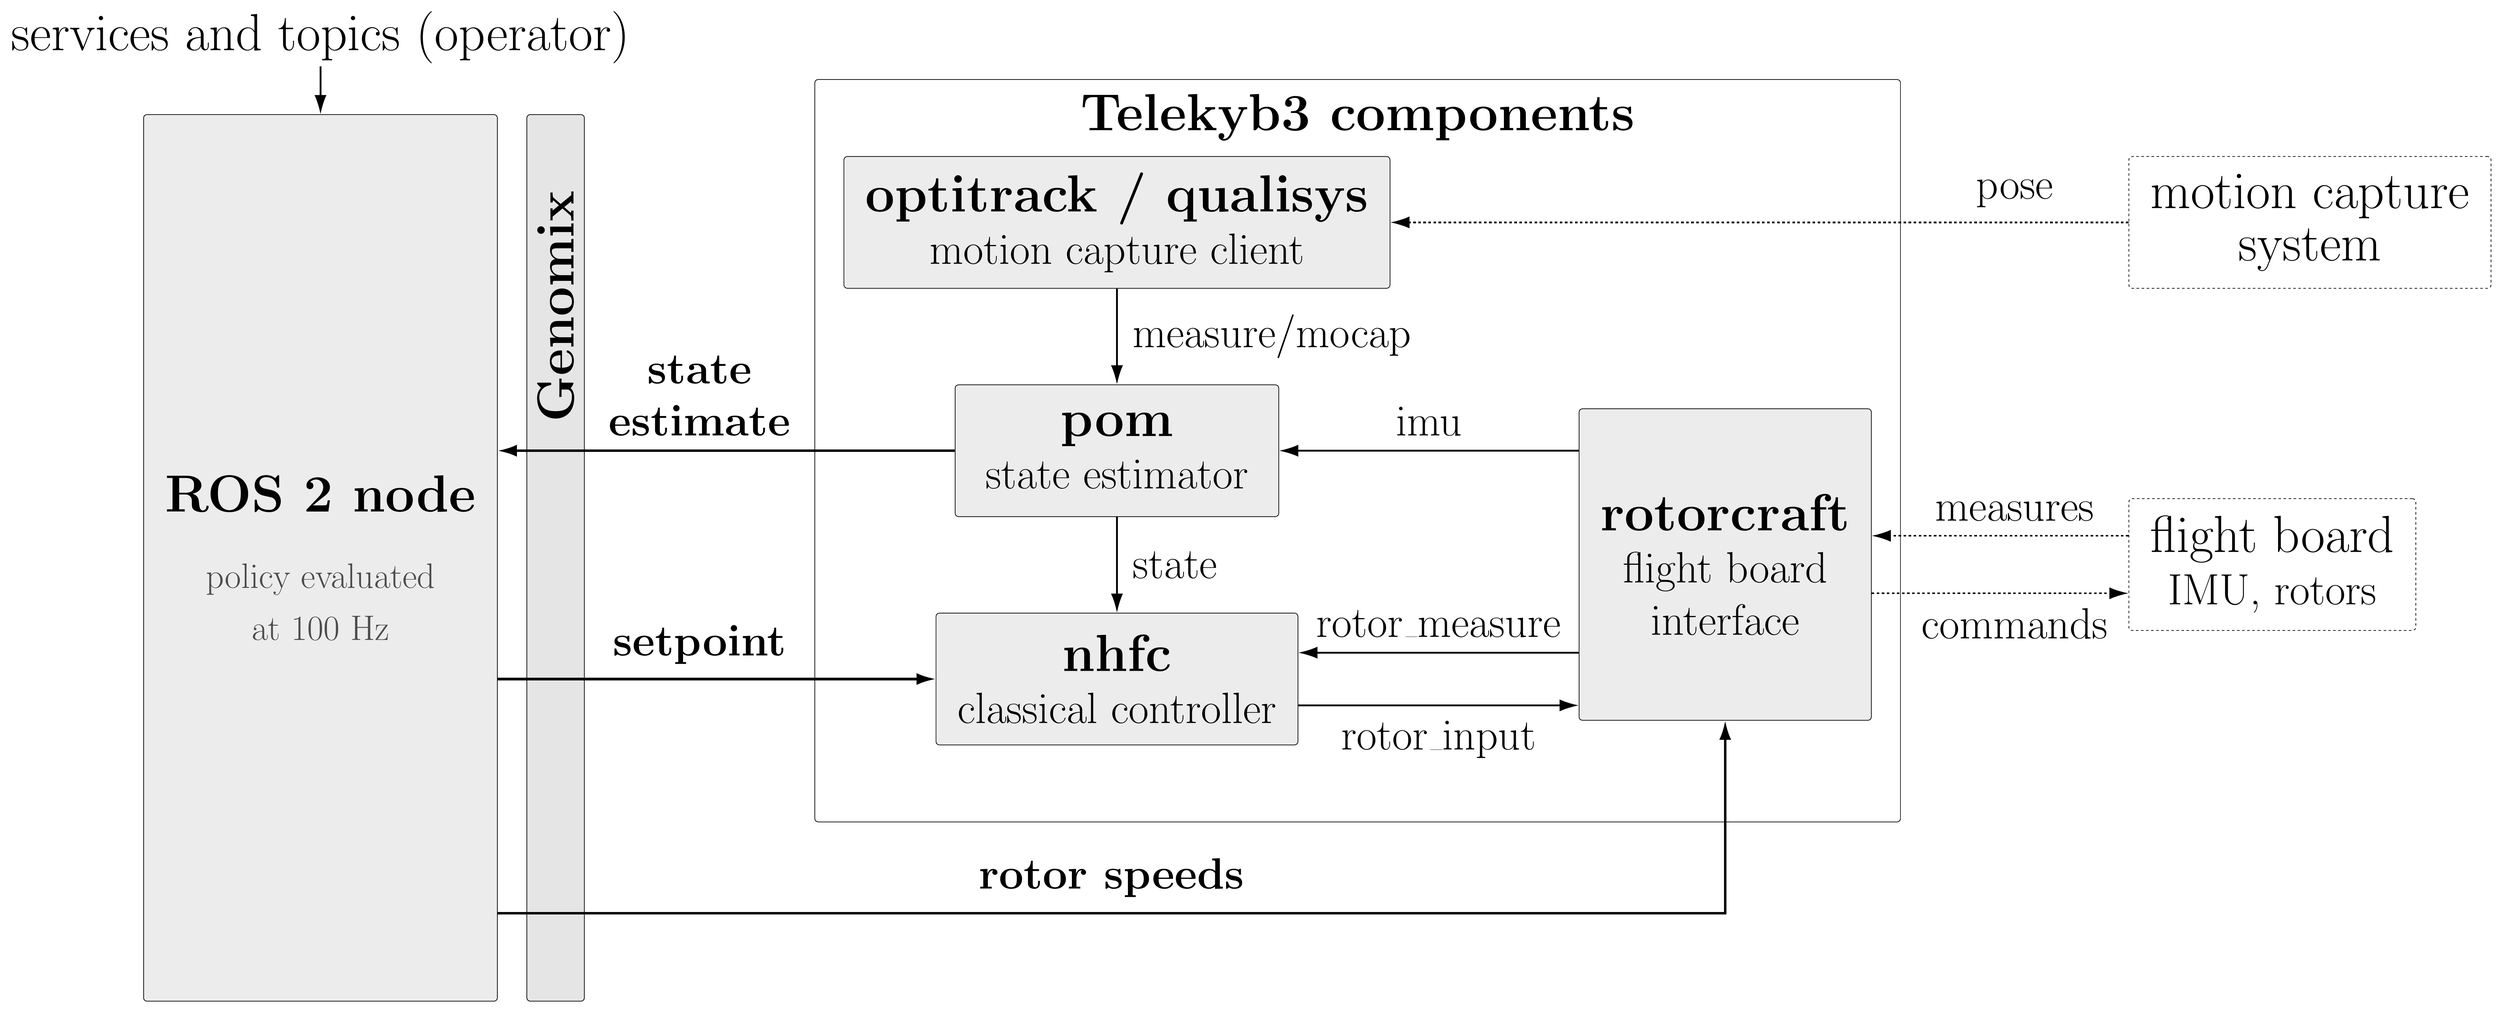
\begin{tikzpicture}[
    >={Latex[length=8mm, width=5mm]}, % Arrows scaled up slightly to match text
    font=\TextSub, % Global base font increased
    block/.style={
        rectangle,
        rounded corners,
        draw,
        thick,
        fill=gray!15,
        text centered,
        align=center,
        inner xsep=0.9cm,
        minimum width=13.5cm,
        minimum height=5.5cm
    },
    container/.style={
        rectangle,
        rounded corners,
        draw,
        thick,
        inner xsep=1.2cm,
        inner ysep=3.2cm
    },
    dashed_block/.style={
        rectangle,
        rounded corners,
        draw,
        thick,
        dashed,
        text centered,
        align=center,
        inner xsep=0.9cm,
        minimum width=10cm,
        minimum height=5.5cm
    },
    arrow/.style={
        ->,
        thick,
        line width=2pt
    },
    dashed_arrow/.style={
        ->,
        dashed,
        thick,
        line width=2pt
    }
]

% ROS 2 Node (taller, so that the rotor speeds arrow leaves from its side)
\node[block, minimum height=37cm, minimum width=12cm, yshift=-5.5cm] (ros2) {
    \textbf{\TextTitle ROS 2 node} \\[1cm]
    \textcolor{black!70}{\TextSmall policy evaluated} \\ \textcolor{black!70}{\TextSmall at 100 Hz}
};

% Operator
\node[above=2cm of ros2, font=\TextTitle] (operator) {services and topics (operator)};
\draw[arrow] (operator) -- (ros2);

% Genomix
\node[block, right=1.2cm of ros2, minimum width=2.4cm, minimum height=37cm, fill=gray!20] (genomix) {};
\node[rotate=90, font=\bfseries\TextTitle] at ([yshift=10.5cm]genomix.center) {Genomix};

% Telekyb3 internal components
\node[block, right=10.8cm of genomix, yshift=14cm] (optitrack) {
    \textbf{\TextTitle optitrack / qualisys} \\ \TextSub motion capture client
};

\node[block, below=4cm of optitrack] (pom) {
    \textbf{\TextTitle pom} \\ \TextSub state estimator
};

\node[block, below=4cm of pom] (nhfc) {
    \textbf{\TextTitle nhfc} \\ \TextSub classical controller
};

\node[block, right=12.5cm of pom, yshift=-4.75cm, minimum height=13cm, minimum width=11cm] (rotorcraft) {
    \textbf{\TextTitle rotorcraft} \\ \TextSub flight board \\ \TextSub interface
};

% Telekyb3 Components container 
\node[container, fit=(optitrack) (pom) (nhfc) (rotorcraft)] (telekyb3) {};
\node[anchor=north, font=\bfseries\TextTitle, yshift=-0.5cm] at (telekyb3.north) {Telekyb3 components};

% External systems 
\node[dashed_block, right=9.5cm of telekyb3.east |- optitrack.center] (mocap) {
    \TextTitle motion capture \\ \TextTitle system
};

\node[dashed_block, right=9.5cm of telekyb3.east |- rotorcraft.center] (flightboard) {
    \TextTitle flight board \\ \TextSub IMU, rotors
};

% --- Connections and Arrows ---

% Mocap -> Optitrack
\draw[dashed_arrow] (mocap.west) -- (optitrack.east);
\node[above=0.5cm, font=\TextSub] at ($(telekyb3.east |- mocap.west)!0.5!(mocap.west)$) {pose};

% Optitrack -> Pom
\draw[arrow] (optitrack.south) -- node[right=0.5cm, font=\TextSub] {measure/mocap} (pom.north);

% Pom -> NHFC
\draw[arrow] (pom.south) -- node[right=0.5cm, font=\TextSub] {state} (nhfc.north);

% Rotorcraft -> Pom
\coordinate (imu_mid) at ($(rotorcraft.west |- pom.east)!0.5!(pom.east)$);
\draw[arrow] (rotorcraft.west |- pom.east) -- (pom.east);
\node[above=0.5cm, font=\TextSub] at (imu_mid) {imu};

% Rotorcraft <-> NHFC 
\draw[arrow] ([yshift=1.1cm]rotorcraft.west |- nhfc.east) -- node[above=0.5cm, font=\TextSub] {rotor\_measure} ([yshift=1.1cm]nhfc.east);
\draw[arrow] ([yshift=-1.1cm]nhfc.east) -- node[below=0.5cm, font=\TextSub] {rotor\_input} ([yshift=-1.1cm]rotorcraft.west |- nhfc.east);

% Rotorcraft <-> Flight board (labels centered in the gap outside the container)
\coordinate (measures_mid) at ($([yshift=1.2cm]telekyb3.east |- rotorcraft.east)!0.5!([yshift=1.2cm]flightboard.west)$);
\draw[dashed_arrow] ([yshift=1.2cm]flightboard.west) -- ([yshift=1.2cm]rotorcraft.east);
\node[above=0.5cm, font=\TextSub] at (measures_mid) {measures};

\coordinate (commands_mid) at ($([yshift=-1.2cm]telekyb3.east |- rotorcraft.east)!0.5!([yshift=-1.2cm]flightboard.west)$);
\draw[dashed_arrow] ([yshift=-1.2cm]rotorcraft.east) -- ([yshift=-1.2cm]flightboard.west);
\node[below=0.5cm, font=\TextSub] at (commands_mid) {commands};

% ROS 2 specific arrows
\coordinate (pom_mid) at ($(genomix.east |- pom.west)!0.5!(telekyb3.west |- pom.west)$);
\coordinate (nhfc_mid) at ($(genomix.east |- nhfc.west)!0.5!(telekyb3.west |- nhfc.west)$);

% state estimate
\draw[arrow, line width=3pt] (pom.west) -- (ros2.east |- pom.west);
\node[above=0.5cm, font=\TextSub, align=center] at (pom_mid) {\textbf{state}\\ \textbf{estimate}};

% setpoint
\draw[arrow, line width=3pt] (ros2.east |- nhfc.west) -- (nhfc.west);
\node[above=0.5cm, font=\TextSub] at (nhfc_mid) {\textbf{setpoint}};

% rotor speeds: leaves the side of the ROS 2 node, crosses Genomix
\path (telekyb3.south) ++(0, -3.8cm) coordinate (bottom_path);
\coordinate (ros2_out) at (ros2.east |- bottom_path);
\coordinate (rotor_in) at (rotorcraft.south);

\draw[arrow, line width=3pt] (ros2_out) -- node[above=0.5cm, font=\TextSub, pos=0.5] {\textbf{rotor speeds}} (rotor_in |- ros2_out) -- (rotor_in);

\end{tikzpicture}
\end{document}